\documentclass[a4paper, 12pt]{article} % Font size (can be 10pt, 11pt or 12pt) and paper size (remove a4paper for US letter paper)

\usepackage[protrusion=true,expansion=true]{microtype} % Better typography
\usepackage{graphicx} % Required for including pictures
\usepackage{wrapfig} % Allows in-line images
\usepackage{german}
\usepackage{url}
\def\UrlBreaks{\do\/\do-} % defines that when a - occurs it can break the url
\usepackage{color}

\usepackage{mathpazo} % Use the Palatino font
\usepackage[T1]{fontenc} % Required for accented characters


\linespread{1.05} % Change line spacing here, Palatino benefits from a slight increase by default

\makeatletter
\renewcommand\@biblabel[1]{\textbf{#1.}} % Change the square brackets for each bibliography item from '[1]' to '1.'
\renewcommand{\@listI}{\itemsep=0pt} % Reduce the space between items in the itemize and enumerate environments and the bibliography

\renewcommand{\maketitle}{ % Customize the title - do not edit title and author name here, see the TITLE block below
\begin{flushright} % Right align
{\LARGE\@title} % Increase the font size of the title

\vspace{50pt} % Some vertical space between the title and author name

{\large\@author} % Author name
\\ \vspace{10pt}\@date % Date

\vspace{40pt} % Some vertical space between the author block and abstract
\end{flushright}
}

%----------------------------------------------------------------------------------------
%	TITLE
%----------------------------------------------------------------------------------------

\title{\textbf{Die Rolle von Social Media im Produktentwicklungsprozess
}\\ % Title
WS 2013\\\vspace{5pt}
Gruppe 6d} % Subtitle

 

 

 
\author{Fink Tobias (0925109)\\
 St"utz Anton (1129424)\\
 \vspace{10pt}
\textbf{}
\\{\textit{}}} % Institution

%----------------------------------------------------------------------------------------

\begin{document}

\maketitle % Print the title section

\newpage

\tableofcontents

\newpage

%----------------------------------------------------------------------------------------
%	ESSAY BODY
%----------------------------------------------------------------------------------------


%%%%%%%%%%%%%%%%%%%%%%%%%%%%%%%%%%%%%
\section{Introduction}
Angelehnt an das  Paper \glqq From Social Media to Social Product Development: The Impact of Social Media on Co-Creation of Innovation'' \textit{(Piller et al. 2012)}\cite{mainreference}, hier und sp"ater nur als das Paper bezeichnet, werden verschiedene Methoden des Co-Creation-Prozesses beschrieben und welche Auswirkungen die wachsende Verbreitung von Social Media auf das Co-Creation hat. Co-Creation wird dabei als Weg zur Nutzung des Innovationspotentials der Konsumenten bezeichnet, in dem man sie in den firmeneigenen Innovationsprozess einbindet. Untermauert wird die theoretische Abarbeitung mit dem Thema durch 3 reale Fallbeispiele.

\subsection{Co-Creation Methoden}
Das Paper beschreibt die Kategorien Sozial Exchange und Market Exchange durch die Art und Form der Belohnung die die Konsumenten durch das Mitwirken an den jeweiligen Methoden erhalten. Sozial Exchange Methoden kennzeichnen sich dabei vor allem durch intrinsische Belohnungen wie Spa\ss{} und weniger durch extrinsische wie Geld, obwohl Anerkennung durch andere Personen oder Firmen schon eine Rolle spielen k\"onnen. Bei Market Exchange ist es genau anders herum. Es wird aber nicht nur eine Unterteilung der Co-Creation Exchange Arten sondern auch der Art der ben"otigten Information durch das Paper vorgenommen.
Auf der einen Seite gibt es Methoden die sich mit den Bed\"urfnissen der Kunden, der sogenannten Need-Information befassen. Wenn man wei"s, was den Kunden zum Kauf motiviert, welche Vorlieben er hat, etc. kann man das Risiko einer Fehlinvestition reduzieren. Auf der anderen Seite versuchen manche Methoden das Know-How, die sogenannte Solution-Information, welche die Kunden haben, auszun\"utzen.
Laut Paper-Information, wie man eine Technologie anwendet um Kundenbed\"urfnisse in Produkte und Dienstleistungen zu verwandeln. 
 Die Methoden lassen sich durch die zwei Dimensionen anhand einer Matrix (Abbildung \ref{coCreationDiagram}) veranschaulichen. Es wird f\"ur jedes der vier Matrixfelder eine Methode besprochen: Toolkits f\"ur User Co-Design, die Lead-User Methode, Ideation Contests und Technical Solution Contests.
\pagebreak
\begin{figure}[h!]
	\caption{Zuordnung der Co-Creation Methoden\cite{mainreference}}
	\centering
		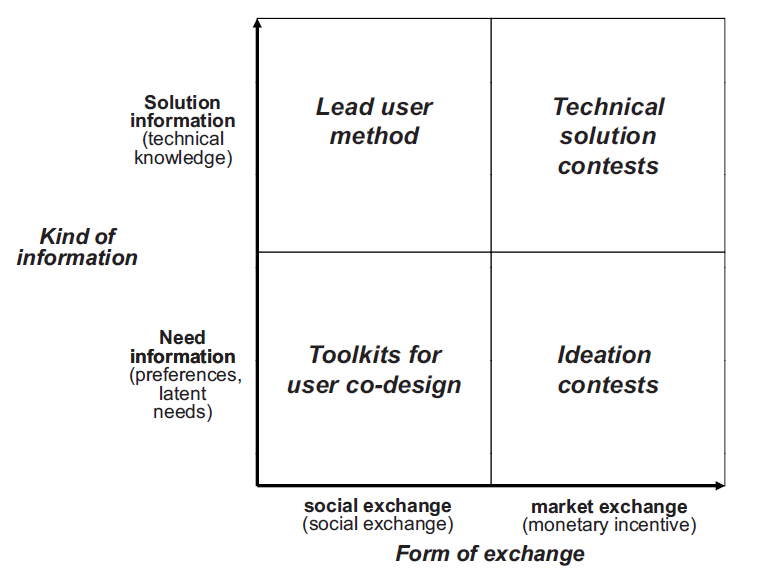
\includegraphics[scale=0.8]{figures/Co-Creation_Matrix}
	\label{coCreationDiagram}
\end{figure}
Das Aufkommen von Sozial Media ver\"andert die Methoden jedoch. Es entstehen neue M\"oglichkeiten aber auch neue Gefahren.  Au\ss{}erdem stellt das Paper die These auf, das die Einteilung der Methoden in Exchange Kategorien etwas verschwimmen werden. D.h. bei Market Exchange Methoden werden intrinsische Belohnungen eine gr\"o\ss{}ere Rolle spielen und umgekehrt bei Sozial Exchange Methoden. Als Erstes befassen wir uns mit den Methoden, die sich durch Sozial Exchange kennzeichnen.
%%%%%%%%%%%%%%%%%%%%%%%%%%%%%%%%%%%%%

%%%%%%%%%%%%%%%%%%%%%%%%%%%%%%%%%%%%%
\section{SocialExchange}
\subsection{Toolkits f\"ur User Co-Design}
Firmen stellen den Konsumenten Toolkits zur Verf\"ugung, damit diese Produkte erstellen oder an ihre Bed\"urfnisse anpassen. Offenere Toolkits gehen dabei eher in erstere Richtung und setzen mehr auf User Innovation. Als Beispiel werden hier Kits zum Erstellen von Computer Chips genannt. Toolkits die den Nutzer nur eine Reihe von austauschbaren Modulen anbieten, gehen eher in die Richtung von User Co-Design und Anpassung. Der Dell Product Configurator ist ein Beispiel daf\"ur. Dadurch, dass die Benutzer es selbst herstellen, erh\"alt das Produkt einen Mehrwert f\"ur sie. Sie sind stolz auf das Ergebnis und m\"ochten es vielleicht auch anderen Leuten zeigen.\\
Toolkits k\"onnen allerdings auch Probleme verursachen. Falls die Auswahlm\"oglichkeiten zu komplex sind, ist der Nutzer eventuell \"uberfordert. Au\ss{}erdem fallen zus\"atzliche Kosten f\"ur Kundensupport an. Social Media kann diesen Problemen vielleicht entgegenwirken. Hilfe kann dadurch auch von Bekannten kommen, was auch hilft komplexe Entscheidungen zu vereinfachen.
Wenn die Produkte der Kunden durch Social Media allerdings mehr im Rampenlicht stehen, k\"onnen Kunden mit popul\"aren Designs auch Ruhm und Geld bekommen. Dadurch r\"uckt der Grund f\"ur die Benutzung eines Toolkits wiederum eher in die Richtung Monetary Incentive und somit die Methode Richtung Market Exchange.\\
Ein Beispiel f\"ur Toolkits w\"are die Webseite \url{www.mymuesli.com}, auf der man aus einer Auswahl von Zutaten w\"ahlen und sein eigenes Muesli kreieren kann. Da jedes Muesli eine ID bekommt, kann es auch von anderen Leuten bestellt werden. Es w\"are denkbar, dass ein Nutzer f\"ur die Schaffung eines beliebten, h\"aufig bestellten Produkts auch belohnt werden k\"onnte.\\
Ein anderes Beispiel w\"aren diverse PC Konfiguratoren, wie der von Ditech\cite{DITECH}. Der Kunde kann aus einer Menge von vorgefertigten PCs w\"ahlen und die eingebauten Teile seinen W\"unschen anpassen. Da sich viele Leute nicht so gut im Hardwarebereich auskennen, wird zus\"atzlich auch noch ein Support Service angeboten. W\"urde Ditech aber eine Einbindung in Facebook erlauben, k\"onnten sich auch Freunde den PC entwurf ansehen und Verbesserungsvorschl\"age machen. Diese w\"urde Ditech sicher Support Kosten ersparen.
\subsection{Lead-User Methode}
Im Paper wird ein Lead User als ein Konsument beschrieben, der bestimmte Bed\"urfnisse fr\"uher hat als der Rest des Marktes und stark vom Erf\"ullen dieser profitiert. Sie haben selbst innovative Ideen, wollen (oder k\"onnen) daraus jedoch keinen monet\"aren Profit machen. Dadurch teilen sie ihre Ideen mit Firmen oder andern Usern, was es den Firmen erm\"oglicht, sie f\"ur bestimmte innovative Probleme heranzuziehen. In solch einem Fall ist es auch nicht ungew\"ohnlich, dass Lead User andere vorschlagen, die sich besser mit einem Problem auskennen - Pyramiding.\\
Social Media macht es einfacher Lead User zu finden. Das hilft klarerweise Firmen, aber auch anderen Lead Usern, weil diese sich besser austauschen k\"onnen und Probleme effizienter l\"osen. Andererseits reduziert Social Media eventuell auch die Entrittsbarrieren des Marktes. Dadurch ist es Lead Useren eventuell doch einfacher m\"oglich mit ihrer Idee Profit zu machen, wodurch sie ein eigenes Unternehmen gr\"unden und nicht ihre Ideen weitergeben. So kann Social Media vielleicht auch zu einem h\"oheren Wettbewerb zwischen Lead Useren und Unternehmen f\"uhren. Weiters steigt auch der Wettbewerb um Lead User, wenn diese einfacher zu finden sind.














%%%%%%%%%%%%%%%%%%%%%%%%%%%%%%%%%%%%%

%%%%%%%%%%%%%%%%%%%%%%%%%%%%%%%%%%%%%
\section{MarketExchange}
\subsection{Technical Solution Contest}
Ein Technical Solution Contest ist ein Wettbewerb bei dem ein Problem an eine gro\ss{}e Anzahl an Personen ausgesendet wird. Dies wird auch als Broadcasting bezeichnet. Die Personen die das Problem l\"osen sollen, werden als Solver bezeichnet und bekommen eine Belohnung wenn ihr L\"osungsvorschlag unter den besten ist. Um mehr Leute zu erreichen, und so an bessere L\"osungen zu kommen, wird oft eine Zwischenfirma beauftragt die sich auf die Suche nach eben diesen spezialisiert hat.\\
Social Media macht es nat\"urlich einfacher mehr Solver f\"ur ein Projekt zu erreichen. Das kann aber auch zum Nachteil der Zwischenfirma werden, denn wenn auch ohne sie eine gro\ss{}e Anzahl f\"ur den Wettbewerb gewonnen werden kann, wer braucht sie noch? Weiters \"andert sich auch das Verh\"altnis zwischen den Teilnehmern, welche sich jetzt gegenseitg beginnen kennenzulernen. So wird aus Einzelarbeit mit nur monet\"arer Belohnung Gruppenarbeit mit vermehrter sozialer Belohnung. Sollten sich die Teilnehmer dadurch gegenseitig positiv Beeinflussen und verstr\"arken kann das gut f\"ur den Zweck des Wettbewerbs sein. Sollte es dadurch allerdings vermehrt zu Trittbrettfahrern in Gruppen kommen und dadurch pro Person zu weniger L\"osungspotential kommen, kann das auch negativ zu bewerten sein.
\subsection{Ideation Contests}
Eine andere Art von Wettbewerb ist der Ideation Contest, der im Gegensatz zum Technical Solution Contest keine L\"osung f\"ur ein technisches Problem sucht, sondern Ideen oder Innovationen basierend auf einer vorgegebenen Aufgabe. Um zur Teilnahme zu motivieren gibt es Preise f\"ur die besten Ergebnisse. Da die Preise aber von eher geringerm Wert und die Anzahl der Teilnehmer hoch ist, spielen soziale Aspekte hier eine gr\"o\ss{}ere Rolle als beim Technical Solution Contest.\\
Wegen der starken \"ahnlichkeit zum  Technical Solution Contest ist die Verwendung von Social Media ungef\"ahr gleich einzusch\"atzen. Da die Kommunikation zwischen den Teilnehmern allerdings noch gemeinschaftlicher ist, k\"onnten Off-Topic Diskussionen in den vom Wettbewerbsveranstalter betriebenen Netzwerken und Foren ein schwerer zu regulierendes Problem werden.
%%%%%%%%%%%%%%%%%%%%%%%%%%%%%%%%%%%%%

%%%%%%%%%%%%%%%%%%%%%%%%%%%%%%%%%%%%%
\section{Fallbeispiele}
Der folgende Abschnitt stellt drei reale Fallbeispiele vor.
\subsection{Quirky}
Quirky ist ein Unternehmen gegr�ndet von Ben Kaufman im Jahr 2009, welches in New York City angesiedelt ist. Die Gesch�ftsidee besteht darin eine �ffentlich zug�ngliche Onlineplattform einzurichten und �ber diese jedem einzelnen die M�glichkeit zu geben Produktideen vorzustellen(fr�her gegen eine Geb�hr). Andere User k�nnen nunmehr die Produktideen bewerten und Kommentieren. Kommen bei einer Produktidee gen�gend positive R�ckmeldungen wird das Produkt gemeinsam mit der Community entwickelt. Hier ist schon zu erkennen, dass die Community einen wichtigen Bestandteil des Unternehmens darstellt. Abbildung \ref{quirkySystem} zeigt den Einfluss der Community noch einmal grafisch. Um eine m�glichst starke Community aufzubauen ben�tigt es nat�rlich Anreize um die einzelnen User an das Unternehmen zu binden. Quirky verfolgt hier ma"sgeblich den monet�ren Ansatz und bietet laut einem Werbeslogan auf ihrer Website schon f�r einen Klick eine finanzielle Verg�tung.
\begin{figure}[h!]
	\caption{�bersicht �ber den Crowdsourcing-Prozess bei Quirky\cite{TENREASONSQUIRKY}}
	\centering
		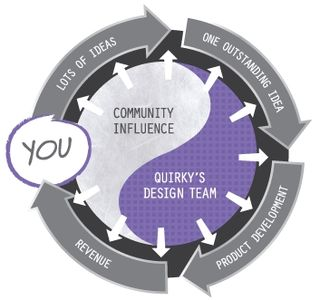
\includegraphics[scale=0.9]{figures/Quirky}
\label{quirkySystem}
\end{figure}

Hierbei ist anzumerken, dass Quirky ein hybrides Modell an Community-Beteiligung und eigener Entwicklung nutzt. Quirky k�mmert sich um die Koordination sowie um die schwierigeren Entwicklungsschritte, wie zum Beispiel die technische Entwicklung des Produkts.

Quirky vertraut bei diesem Gesch�ftsmodell haupts�chlich auf die sogenannten Lead-User, welche in den vorangegangen Kapiteln genauer beschrieben wurden. Eine neue Idee einzureichen ist relativ einfach m�glich �ber die angebotene Online-Plattform(\url{www.quirky.com}). Es wird ein Titel, eine sogenannte \glqq Elevator Pitch\grqq (kurze Beschreibung des Produkts), eine Einteilung in eine von insgesamt 8 Kategorien. Anschlie"send ist zu beantworten welches Problem die Idee l�st und wie das Problem gel�st werden kann.

Ein anderer wichtiger Teil bei der Produktentwicklung ist die Beeinflussung der urspr�nglichen Produktidee �ber die Onlineplattform durch die anderen Community-Mitglieder. Hierf�r wurde von Quirky ein System entwickelt mit sogenannten Influence-Punkten, welche prozentuell vergeben werden. Diese Influence-Punkte geben an inwieweit ein User die Entwicklung eines Produktes beeinflusst hat. Entsprechend dieser Verteilung erfolgt die Aufteilung der Gewinne die mit dem Produkt gemacht werden. Zu beachten ist jedoch, dass man nur Aussicht auf eine finanzielle Verg�tung besitzt, falls das Produkt auch wirklich auf den Markt gebracht wird. Insgesamt sch�ttet Quirky 10\% des Gewinns welches mit dem Produkt gemacht wird an seine Community aus. In Abbildung \ref{quirkyInfluence} wird noch einmal verdeutlicht wie die Influence-Punkte auf die Community aufgeteilt werden.

\begin{figure}[h!]
	\caption{Aufteilung der Influence-Punkte auf die einzelnen Entwicklungsstufen\cite{QUIRKYCOMINF}}
	\centering
		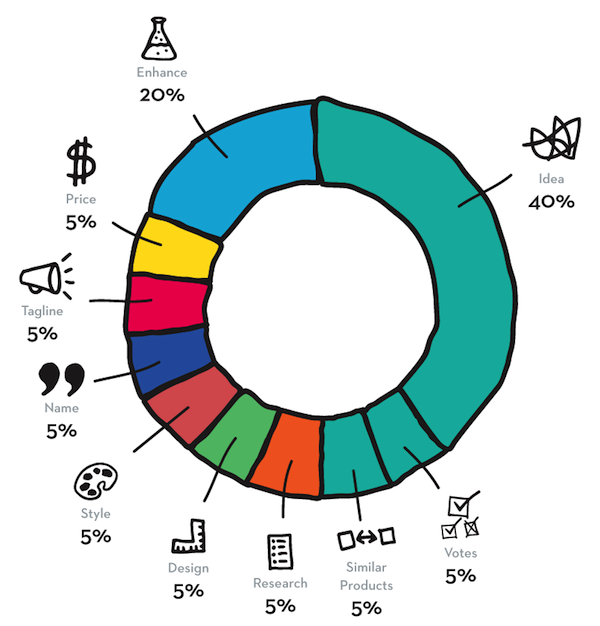
\includegraphics[scale=0.8]{figures/influence-chart1}
	\label{quirkyInfluence}
\end{figure}

Ein Nachteil der finanziellen Verg�tung in der Form wie sie Quirky anwendet, bei der man bei jeder Interaktion mit der Community Geld verdient ist, dass es zwar viele Interaktionen der Community gibt, jedoch die Qualit�t der Kommentare, Votings(man voted f�r das bereits beste Produkt) fraglich ist. Quirky scheint dieses Problem jedoch nicht zu haben.

Ein weiteres Problem stellt die Abtretung der Rechte des Lead-Users dar, falls die Produktidee von Quirky angenommen wird. Es besteht zwar ein Anspruch auf eine entsprechende Verg�tung durch Quirky, jedoch wenn Patente angemeldet werden ist es fraglich wer als Erfinder eingetragen wird. Oftmals werden Produktideen von mehr als 800 Personen beeinflusst. Hier stellt sich die Frage ob nicht Plattformen wie Kickstarter und co. besser geeignet sind gute Ideen umzusetzen und zu finanzieren, da hier die Rechte bei den Erfindern bleiben.
\cite{LOSINGRIGHTS}

Quirky hat mit Stand Dezember 2013 eine globale Community von 600000 Mitgliedern, die Produkte entwerfen und beeinflussen.\cite{REPORTQUIRKY2345}


\subsection{InnoCentive}
InnoCentive st�tzt sich �hnlich wie Quirky auf eine kollaborative Onlineplattform, jedoch konzentriert sich InnoCentive nicht auf die Entwicklung neuer Produkte sondern auf die L"osung von Problemen in wissenschaftlichen Bereichen wie zum Beispiel der Informatik, Mathematik und Chemie. Jede Person kann sich bei dieser Plattform anmelden und zur L�sung eines Problems beitragen, falls durch den eingebrachten L�sungsvorschlag das Problem gel�st werden konnte wird ein Preisgeld an den jeweiligen User entrichtet. F�r jede ver�ffentlichte sogenannte Challenge verrechnet InnoCentive eine Geb�hr in der H�he von ungef�hr 20000\$\cite{WIKIINNOCENTIVE}. Hier ist schon zu erkennen, dass das Gesch�ftsmodell darauf ausgerichtet ist Firmen zu erm�glichen Probleme zu posten, die sie firmenintern nur sehr schwer oder nur mit einem finanziell viel h�herem Aufwand l�sen k�nnen.

\subsection{Crowdspirit}
\glqq CrowdSpirit is a platform connecting companies with innovators to help with the design of products and services.\grqq\cite{OPENBUSINESS4711}

Crowdspirit hat eine gro"se �hnlichkeit zu den zwei obigen Fallbeispielen, mit dem gro"sen Unterschied, dass es gescheitert ist. 

Folgenden Fehler macht man heute f�r das Scheitern verantwortlich:
Organisatorische Probleme mit der Community, da sich die Community zu wenig beteiligt hat musste in Folge sogar das Gesch�ftsmodell angepasst werden. Jedoch ohne langfristigen Erfolg. Hier kann man auch klar erkennen, dass die Motivation der Community ein wesentlicher Bestandteil des Gesch�ftsmodells sein muss. In Folge wurden zwar viele Ideen auf der Onlineplattform gesammelt, jedoch kam es nie wirklich zu einem co-creation Prozess. Ein weiteres Problem war die Einstellung des CEOs, welcher sich zu sehr auf den nationalen franz�sischen Markt konzentriert hat, anstatt internationales Publikum anzusprechen.
\cite{LESSONSFROMFAILURE}














%%%%%%%%%%%%%%%%%%%%%%%%%%%%%%%%%%%%%

%%%%%%%%%%%%%%%%%%%%%%%%%%%%%%%%%%%%%
\section{Conclusion}
Unserer Meinung nach hat Social Media im Produktentwicklungsprozess gro"ses Potential, wenn man es zum richtigen Zeitpunkt und in der richtigen \glqq Dosis\grqq anwendet. Social Media macht es einfach eine gro"se Bandbreite von Personen anzusprechen, die in den verschiedensten Bereichen t"atig sind und so einen breitgef"acherten Erfahrungsschatz mitbringen. Jedoch hat die Erfahrung gezeigt, dass die Community auch richtig motiviert werden muss, damit sie bereit ist konstruktive Beitr"age bei dem Produktentwicklungsprozess zu leisten.
%%%%%%%%%%%%%%%%%%%%%%%%%%%%%%%%%%%%%

\bibliographystyle{unsrt}

\bibliography{references}

%----------------------------------------------------------------------------------------

\end{document}
